% Auf ungerader Seite starten
\cleardoublepage

%%%%%%%%%%%%%%%%%%%%%%%%%%%%%%%%%%%%%%%%%%%%%%%%%%%%%%%%%%%%%%%%%%%%%%%%%%%%%%%%%%%%%%%%%
% Einleitung
%%%%%%%%%%%%%%%%%%%%%%%%%%%%%%%%%%%%%%%%%%%%%%%%%%%%%%%%%%%%%%%%%%%%%%%%%%%%%%%%%%%%%%%%%

\chapter{Introduction}
\label{Chapter: Introduction}

Turbofan engines are widely used in commercial aircraft.  New, more stringent requirements with regards to emissions, fuel consumption and noise pollution are putting pressure on aircraft engine manufacturers to increase the efficiency of their products. From a technical point of view, there are two options: increase the thermal efficiency of the turbine stage or increase the bypass ratio of the engine. The bypass ratio is the amount of air that passes around the turbine core rather than through it.  Generally, a higher bypass ratio results in a quieter, more efficient engine. To increase the bypass ratio, the diameter of the engine's fan blades must be increased.  However, increasing the fan diameter leads to an increase in the circumferential velocity of the fan blade tips.  At very high speeds, large increases in losses and noise emissions are observed.

In conventional turbofans, the fan and the low-pressure compressor and turbine which drives the fan are attached to single shaft.  In this configuration, the speed of the compressor stage is limited by the blade tip speeds to the fan.  With the addition of a gearbox between the fan and the compressor and turbine, the fan speed can be greatly reduced while the compressor and turbine can rotate much faster.  Both components can therefore operate at their optimal speeds, greatly increasing efficiency and reducing noise.

However, geared turbofans are not without drawbacks.  In addition to increased complexity and manufacturing cost, a significant amount of energy is lost as heat within the gearbox.  The cooling and lubrication of the gearbox are key challenges.  These functions are realized with oil jets arranged around the gears.  The interaction between the oil jets and the gear surfaces determines the cooling and lubrication performance as well as the further propagation of the oil within the gearbox.

Therefore, this interaction is a current focus of research at the Insitute of Thermal Turbomachinery at the Karlsruhe Institute of Technology.  Experimental investigations in this area are difficult due to the small time scale and inaccessible location of the interactions. However, Computational Fluid Dynamics (CFD) methods offer possibilities for detailed investigation. One such method is Smoothed Particle Hydrodynamics (SPH), a particle-based method that is well-suited to modeling free surface flows and moving boundaries.  SPH, like other approaches to fluid dynamics modeling, is very computationally expensive.

It is desirable to reduce the required computation time as much as possible. For this purpose, this work examines an approach to increasing the computational efficiency of the SPH solver and therefore reducing the required computation time. 

\chapter{Objective}

\section{Motivation}
\label{SECTION:Motivation}
Smoothed-particle hydrodynamics is a computational method which can be used to simulate mechanics of solids and fluids.  It is mesh-free and employs the Lagrangian approach, which makes it well-suited for complex problems with free surface flows and moving boundaries.

Compared to mesh-based methods, SPH requires a very large number of particles to ensure an equivalent resolution.  However, in applications where there is relatively little high-density fluid (e.g.  oil) in a computational space filled with low-density fluid (e.g.  air), the low-density phase cam be completely omitted.  This is results in a sparse computational domain, in which the amount of particles is small compared to the size of the domain.

During an SPH-method simulation, particles interact locally within a characteristic radius ("smoothing length").  In other words, each particle's behavior is influenced only by the particles surrounding it within a certain range.  Therefore, for each particle $p_i$ in the domain, all points within a certain cut-off radius $r$ around the particle must be determined.  This type of search is called {\itshape fixed-radius near neighbor} (frNN) search.

In the in-house code currently in use at the Insitute for Thermal Turbomachinery, the fixed-radius near neighbors search is implemented using cell linked-lists (CLL, also cell lists). In sparsely-filled computational domains as seen in simulations using the SPH method, other methods for frNN search may yield a performance advantage over the CLL method, in the form of reduced run time or decreased memory use.

\section{Problem}
\label{SECTION:Problem}
The fixed-radius near-neighbor search in this case is specified as follows:

{\itshape
For each point $p_i$ within the computational domain, find all neighbors $p_j$ that lie less than a cut-off radius $r = 3d_x$ , away from the particle, where $d_x$ is the mean particle spacing. This includes the particle $p_1$itself. The result is a set of interactions $p_i \leftrightarrow p_j$, where  $p_j \leftrightarrow p_i $ is considered identical to $p_i \leftrightarrow p_j$ and is not repeated.}

\section{Objective}
\label{SECTION:Objective}
The objective of this work is to compare alternative methods for solving the described fixed-radius near neighbor search problem to the existing solution using CLL. For this purpose, a benchmarking framework is created in which the a comparison can take place independently of the rest of the SPH code. Alternative solutions are researched and the most promising methods are implemented within the framework along with the CLL method. The benchmarks measure process runtime and memory use, which are then used to compare the search methods.

\chapter{Neighbor Search Methods}

The following sections describe tools that can be used to solve the fixed-radius near neighbor search problem described in section~\ref{SECTION:Problem}. These are implemented in C++ 11 and outfitted with timing code in order to measure their execution times. 

\section{Cell Linked-Lists Method}

The cell-linked lists method (also called linked-cell method or cell-lists method) divides the calculation domain into cells of edge lengths equal to or greater than the cutoff radius of the interaction search. Therefore, to find the neighbors of a particle, only the cells adjacent to the cell containing the particle must be searched. In the 3D case, the potential neighbors of a particle are found within the 27 cells directly surrounding the particle (\cite{Weygand18}).

The particles themselves are first sorted into two lists, $first$ and $next$. The list $first$ contains the indices of the first particle in the cell for each cell, i.e.\ $first[i]$ is the first particle in the  $i$-th cell.   The list $next$ links a particle $i$ to the index of the next particle $j$ in the same cell, i.e. $next[i] = j$. If there are no further particles in the cell, $next$ contains $-1$. In this manner, by starting with the first particle and following the links until the next index is $-1$, all particles in a cell can be visited in an efficient manner.

To create particle interaction lists for the full domain, the search loops through each cell pair. A cell pair is the current cell and itself, or the current cell and an adjacent cell. For each particle in the current cell, the distance to each particle in the other cell is calculated. If the distance is smaller than the cutoff radius, the interaction is added to the interaction pair lists. For increased efficiency, there is no need to check ``backwards'' into previous adjacent cells, as any interactions between the current cell and the previous cell have already been found.

\section{The {\itshape ANN} Library}
\label{SECTION:ANN}


The ANN library, written by David M. Mount and Sinul Arya (\ref{ANN10}), implements k-nearest neighbor search using methods based on orthogonal space decomposition. The particles in the search domain are spatially sorted into special data structures. ANN supports kd-trees and box-decomposition trees (bd-tress). The bd-tree includes more decomposition methods than the kd-tree and is more robust for highly clustered data sets. 

ANN supports exact and approximate nearest neighbor searching and a number and a number of distance metrics. In this case, the ANN library is used to perform exact fixed-radius NN searching using the Euclidean ($L_2$) distance metric. Exact searches can be performed by setting the tolerance $\epsilon$ to 0. For fixed-radius searching, ANN provides a procedure $annkFRSearch$, which returns the $k$ closest points that lie within the radius bound. Because ANN statically allocates its arrays, the $annFRSearch$ function must be called twice to find all points within the radius: once to find the number of points within the radius, and a second time to actually find the points.

The procedure as implemented in this work is therefore as follows:  First, the search tree structure is initialized using the all data points (particles) in the search domain. Then the $annkFRSearch$ procedure is called twice for each data point. Initially, a search is performed using $annkFRSearch$ with $k = 0$ to find the number of points $k'$ that lie within the radius bound.  Then, the appropriate arrays of size $k'$ are allocated, and filled by calling the procedure a second time with $k = k'$. At this point, the neighbors and therefore the interactions of the current point are known. These must then be inserted into the interaction lists, making sure not to duplicate any interactions.

If there is a known upper bound on the possible number of points within the search radius, it would be possible to pre-allocate arrays that are as large as the upper bound, and therefore need to perform the search only once. It is assumed that this would come at the cost of higher memory use, but it was not tested in the scope of this work. For more detailed information about the ANN libraby, see the ANN Programming Manual (\ref{ANN10}).

\section{The {\itshape nanoflann} Library}
\label{SECTION:NanoFLANN}
{\itshape nanoflann} is a header-only library for C++11 for KD-Tree structures.  It does not support approximate nearest neighbors search.  It includes a number of optimizations for increased efficiency.  For instance, there are no provisions for choosing between or adding custom NN-search algorithms, and by using STL containers for the output data, there is no need to call the fixed-radius search method twice, as is the case with ANN. \ref{FIXME}.

These optimizations could lead to performance advantages of {\itshape nanoflann} over the {\itshape ANN} library. It is also able to work with dynamic point clouds without rebuilding the entire kd-tree index. For these reasons, it could be promising for the final application and is mentioned here and included in the source files. However, a comparison to the ANN library is not included in this report.


\chapter{Project Structure and Requirements}

This chapter describes the structure of the project. First the overall organization and then the individual components are explained. Following that, the prerequisites and processes for building and/or running the code used in various parts of the project are briefly described.

\section{Requirements}
\label{SECTION:REQS}
This project requires a Linux system with {\itshape gcc}, {\itshape bash}, and a recent version of Python 3 with the {\itshape numpy} package to run the benchmarks. Additional Python packages are required to view and execute the analysis notebooks. {\itshape Jupyter Notebook}, {\itshape matplotlib},  {\itshape pandas}, and {\itshape seaborne} can be installed using the python package installer {\itshape pip}. Note: Jupyter requires at least Python 3.3.

\section{Directory Structure}
Figure \ref{FIG:folders} shows the file structure of the project.  First of all, the documentation (i.e.  this pdf) is in the {\itshape docs} folder, and the latex source files are in {\itshape latex}. The {\itshape ann\_1.2.2} directory contains the neighbor search C++ libraries that is examined. The {\itshape nanoflann} directory is an additional neighbor search libraray (see section \ref{FIXME}.  The folders {\itshape src} and {\itshape bin} contain the C++ source files (described in section \ref{SECTION:SRC}) and their compiled binaries, respectively.  The {\itshape scripts} directory is home to the test case generation scripts (described in section \ref{SECTION:TESTS}) and test execution scripts (see Chapter \ref{CHAPTER:BENCHMARKING}).  The {\itshape test} directory contains the working directories of the test runs and the result data.   Finally, the folder {\itshape analysis} contains the iPython notebooks that were used in the examination and analysis of the results.  These are described in more detail in section \ref{SECTION:NOTEBOOKS}.

\begin{figure}[h]
	\centering
	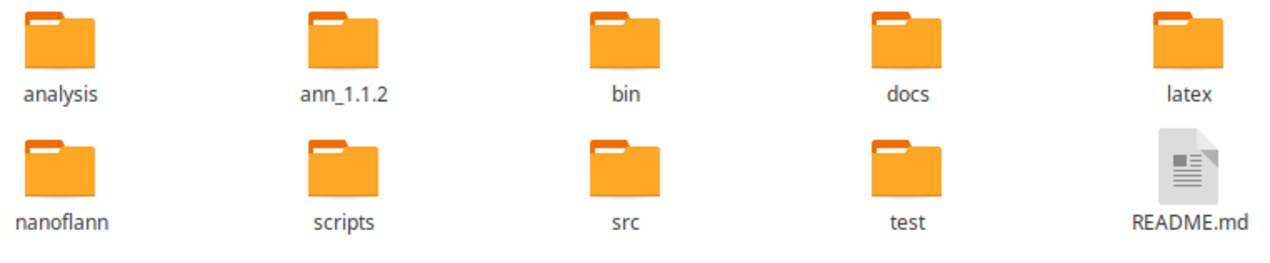
\includegraphics[width=0.75\textwidth]{figures/project_folders.pdf}
	\caption{The root-level structure of the project repository.}
      \label{FIG:folders}
\end{figure}

\section{Search Methods}
\label{SECTION:SRC}

The nearest neighbor search methods are implemented in C++ 11. The {\itshape src} directory contains the source files. The linked-cell method is implemented in {\itshape fr\_cellLinkedList.cpp}. For the ANN method, there are multiple variants. First, {\itshape fr\_ann\_query.cpp} will only query a query single point for its neighbors. For the full nearest neighbor search, a method that builds the interaction pair lists ({\itshape fr\_ann.cpp}) and a method that skips this step ({\itshape fr\_ann\_nolist.cpp}) are provided. This was necessary due to the extremely long time required for generating the interaction pair lists.

The {\itshape src} directory also contains a Makefile which can be used to build any or all of the source files. The resulting executable files are placed in the {\itshape bin} directory upon a successful build. Finally, source files for the Nanoflann library are provided ({\itshape fr\_nanoflann.cpp} and {\itshape utils.h}) for possible future work evaluating this additional  nearest neighbor search method. For more details about Nanoflann, see section \ref{SECTION:NanoFLANN}.

\section{Test Case Scripts}
\label{SECTION:TESTCASESCRIPTS}

To be able to evaluate the performance of the different nearest neighbor search algorithms, a number of different test cases are required. These take the form of a list of data points which are processed by the search method executable. The test cases differ by the distribution of the data points in the search domain and are described in detail in section \ref{FIXME}.

To generate the test cases, different scripts are used. Python was chosen as the scripting language due to familiarity and the availability of easy-to-use plotting libraries for visualization of the data point distributions. In the {\itshape scripts} directory, test case scripts are provided for four different distribution types examined in this work. With the exception of {\itshape test3d\_full}, which simply generates a filled domain, each of the scripts take certain parameters which control the fill and spacing of the points.

The test case scripts are meant to be run within the benchmarking framework, as they also generate a statistics file for later use in the analysis. However, the scripts can also be run separately. Copy the script and the file {\itshape config.py} anywhere and execute the test case script with the Python interpreter. The data points are written to {\itshape data.pts} and can be visualized in 2D or 3D with scripts {\itshape plot\_2d.py} and {\itshape plot\_3d.py}.

\section{Jupyter Notebooks for Analysis}
\label{SECTION:NOTEBOOKS}

To examine and compare the test results, Python is again used in the form of Jupyter Notebooks found in the {\itshape analysis} directory. To access the notebooks, make sure to have the appropriate packages installed (see \ref{SECTION:REQS}). The Jupyter Notebook server can be started from the project root with $jupyter notebook$ and notebooks are viewed and executed via a web browser.

The notebook files themselves are generally self explanatory. The overall structure of the analysis is as follows. In the data-preparation notebook, data is read from the results files in the {\itshape tests} directory, cleaned and labeled, and then written to a CSV file. The following notebooks read the nicely-formatted data from the CSV file and generate various tables and plots. In other words, if the data in the {\itshape tests} directory changes, the data-preparation notebook must be rerun in order to update the CSV file.

\chapter{Test Cases \& Benchmarking Methodology}
\label{CHAPTER:BENCHMARKING}

\section{Running Tests}
\label{SECTION:TESTS}

\begin{figure}[h]
	\centering
	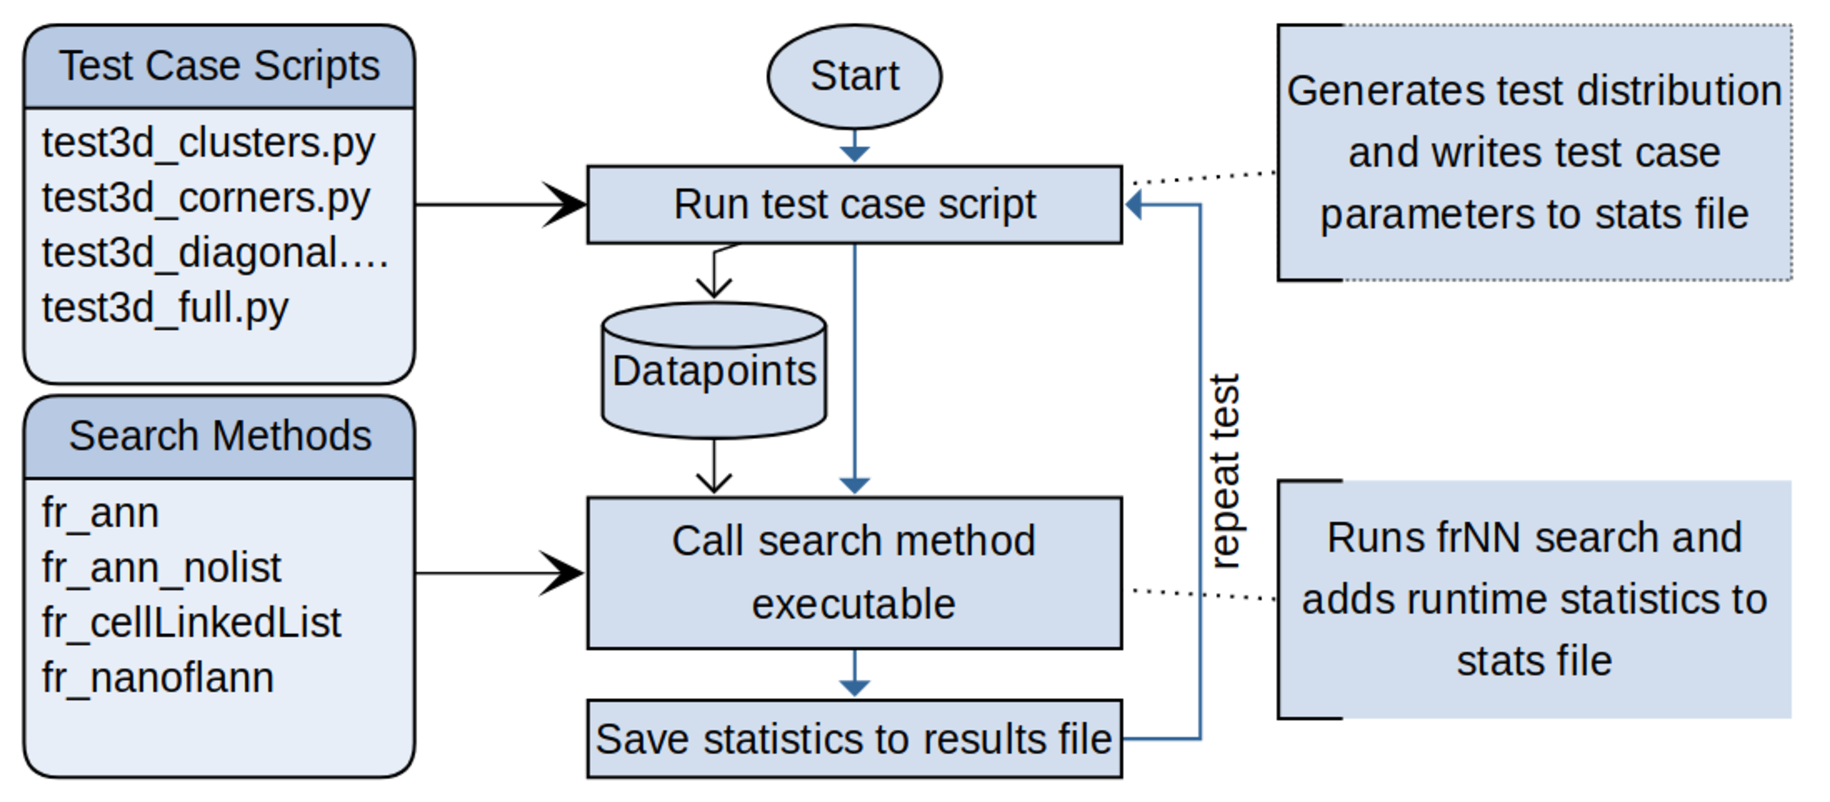
\includegraphics[width=0.75\textwidth]{figures/flowdiagram.pdf}
	\caption{The program flow for a test run with a certain test case and search method.}
\end{figure}


\section{Test Cases}

\section{Benchmarking}

Allows selection of list generation method. Initial tests comparing two list generation methods, it was clear that method1 (FIXME explain!) was about twice as fastas method0 (FIXME: explain). therefore the tests were completed with method 1. While method 0 gnerate 

\chapter{Results and Discussion}

\begin{table}[htbp]
	\centering
	\renewcommand{\arraystretch}{1.3} % Größerer Zeilenabstand
	\captionabove{Results (mean values)}
      \begin{tabular}{lllrrrrrr}
\toprule
    &      &     &  Datapts &  Memory &  $t_{frsearch}$ &  $t_{tksearch}$ &  $t_{processing}$ &  $t_{total}$ \\
fill & filltype & method &          &         &                 &                 &                   &              \\
\midrule
2 & corners & ANN &     7200 &   16.02 &            0.09 &            0.13 &             63.17 &        63.40 \\
    &      & ANN-NL &     7200 &   13.93 &            0.07 &            0.07 &              0.00 &         0.15 \\
    &      & CLL &     7200 &    8.84 &            0.00 &            0.00 &              0.00 &         0.02 \\[2.0ex]
11 & clusters2 & ANN &    27648 &   42.46 &            0.32 &            0.53 &            791.79 &       792.70 \\
    &      & ANN-NL &    27648 &   34.55 &            0.20 &            0.22 &              0.00 &         0.47 \\
    &      & CLL &    27648 &   19.18 &            0.00 &            0.00 &              0.00 &         0.08 \\
    & clusters4 & ANN &    27648 &   34.30 &            0.22 &            0.41 &            441.36 &       442.04 \\
    &      & ANN-NL &    27648 &   28.62 &            0.13 &            0.15 &              0.00 &         0.33 \\
    &      & CLL &    27648 &   13.50 &            0.00 &            0.00 &              0.00 &         0.07 \\
    & clusters6 & ANN &    27648 &   27.53 &            0.14 &            0.26 &            223.46 &       223.92 \\
    &      & ANN-NL &    27648 &   23.46 &            0.08 &            0.11 &              0.00 &         0.23 \\
    &      & CLL &    27648 &   13.03 &            0.00 &            0.00 &              0.00 &         0.07 \\
    & corners & ANN &    28158 &   51.01 &            0.45 &            0.70 &           1339.18 &      1340.39 \\
    &      & ANN-NL &    28158 &   41.14 &            0.28 &            0.28 &              0.00 &         0.62 \\
    &      & CLL &    28158 &   19.25 &            0.00 &            0.00 &              0.00 &         0.08 \\
    & diagonal & ANN &    29424 &   48.75 &            0.41 &            0.67 &           1170.92 &      1172.07 \\
    &      & ANN-NL &    29424 &   39.53 &            0.28 &            0.28 &              0.00 &         0.61 \\
    &      & CLL &    29424 &   19.27 &            0.00 &            0.00 &              0.00 &         0.08 \\[2.0ex]
14 & corners & ANN-NL &    37044 &   52.37 &            0.48 &            0.47 &              0.00 &         1.04 \\
    &      & CLL &    37044 &   20.88 &            0.00 &            0.00 &              0.00 &         0.10 \\[2.0ex]
51 & clusters10 & ANN-NL &   128000 &  111.68 &            0.71 &            0.89 &              0.00 &         1.81 \\
    &      & CLL &   128000 &   41.08 &            0.00 &            0.00 &              0.00 &         0.62 \\
    & clusters20 & ANN-NL &   128000 &  107.62 &            0.67 &            0.87 &              0.00 &         1.75 \\
    &      & CLL &   128000 &   40.04 &            0.00 &            0.00 &              0.00 &         0.60 \\
    & clusters5 & ANN-NL &   128000 &  130.79 &            0.87 &            0.99 &              0.00 &         2.07 \\
    &      & CLL &   128000 &   61.42 &            0.00 &            0.00 &              0.00 &         0.64 \\[2.0ex]
100 & full & ANN-NL &   250000 &  347.17 &            2.88 &            2.80 &              0.01 &         6.09 \\
    &      & CLL &   250000 &  116.75 &            0.00 &            0.00 &              0.00 &         2.14 \\
\bottomrule
\end{tabular}

\end{table}


\begin{figure}[h]
	\centering
	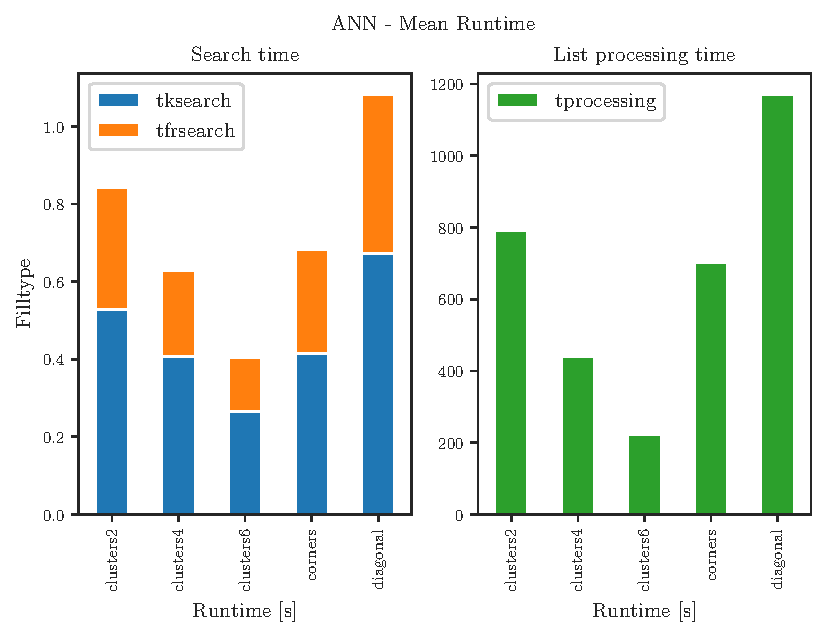
\includegraphics[width=\textwidth]{figures/ann_splitruntime.pdf}
	\caption{FIXME!}
\end{figure}

\begin{figure}[h]
	\centering
	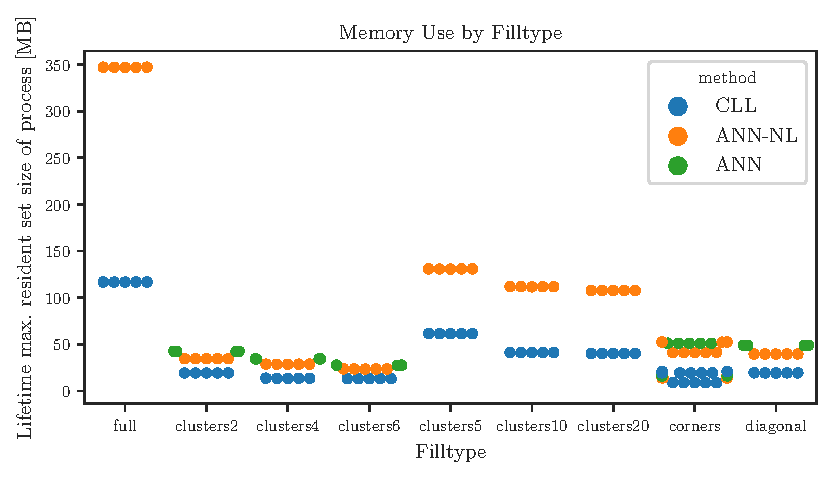
\includegraphics[width=\textwidth]{figures/memory_all.pdf}
	\caption{FIXME!}
\end{figure}
\begin{figure}[h]
	\centering
	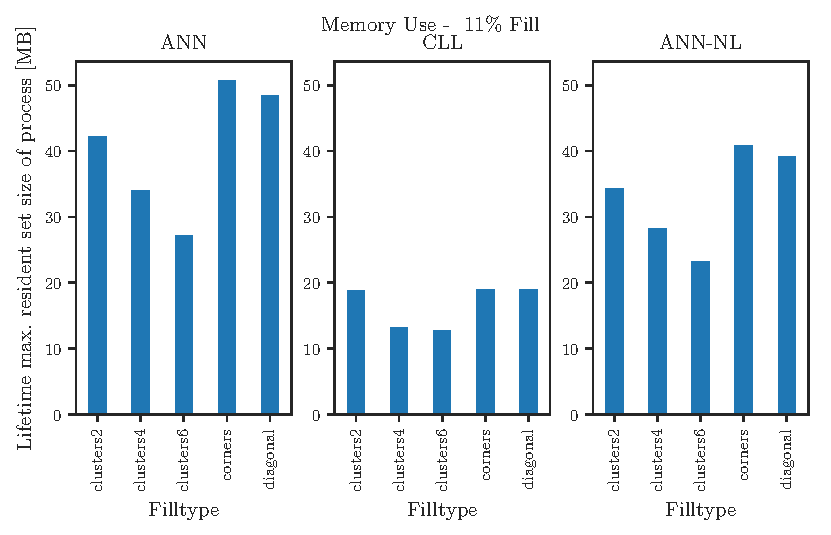
\includegraphics[width=\textwidth]{figures/memory_fill11.pdf}
	\caption{FIXME!}
\end{figure}
\begin{figure}[h]
	\centering
	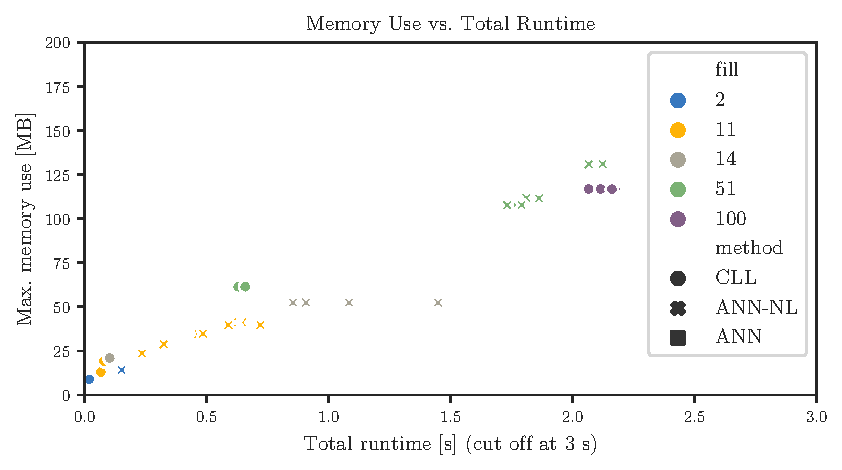
\includegraphics[width=\textwidth]{figures/memory_vs_totalruntime.pdf}
	\caption{FIXME!}
\end{figure}
\begin{figure}[h]
	\centering
	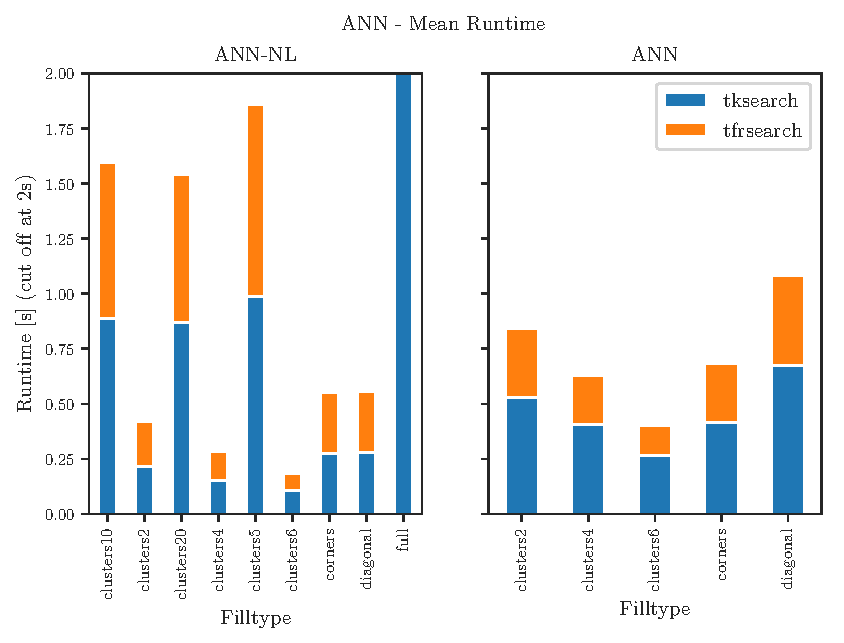
\includegraphics[width=\textwidth]{figures/runtime_ann_annnl.pdf}
	\caption{FIXME!}
\end{figure}
\begin{figure}[h]
	\centering
	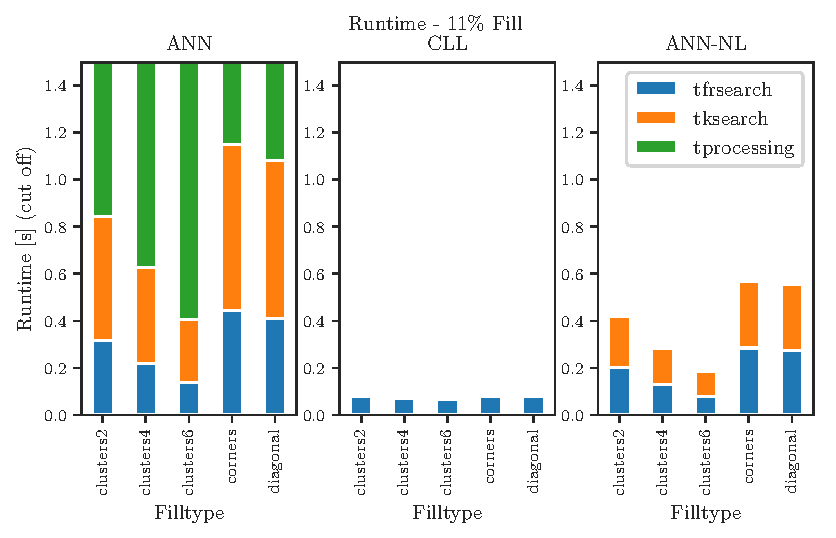
\includegraphics[width=\textwidth]{figures/runtime_fill11.pdf}
	\caption{FIXME!}
\end{figure}

\begin{figure}[h]
	\centering
	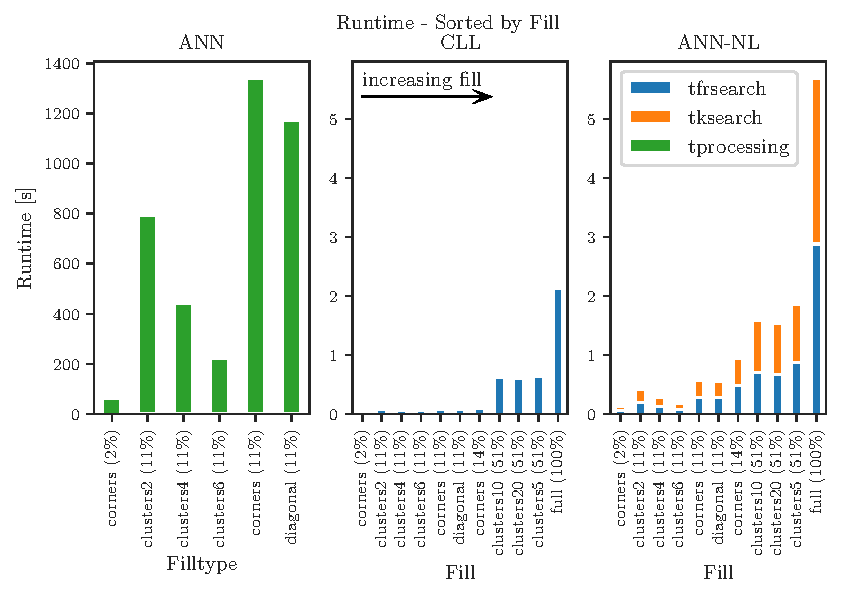
\includegraphics[width=\textwidth]{figures/runtime_filltypes.pdf}
	\caption{FIXME!}
\end{figure}

\begin{figure}[h]
	\centering
	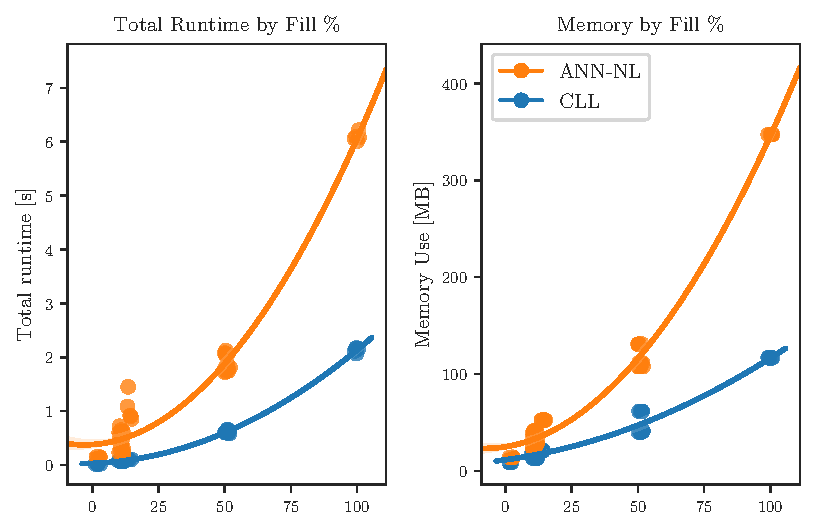
\includegraphics[width=\textwidth]{figures/runtime_vs_fill.pdf}
	\caption{FIXME!}
\end{figure}
\begin{figure}[h]
	\centering
	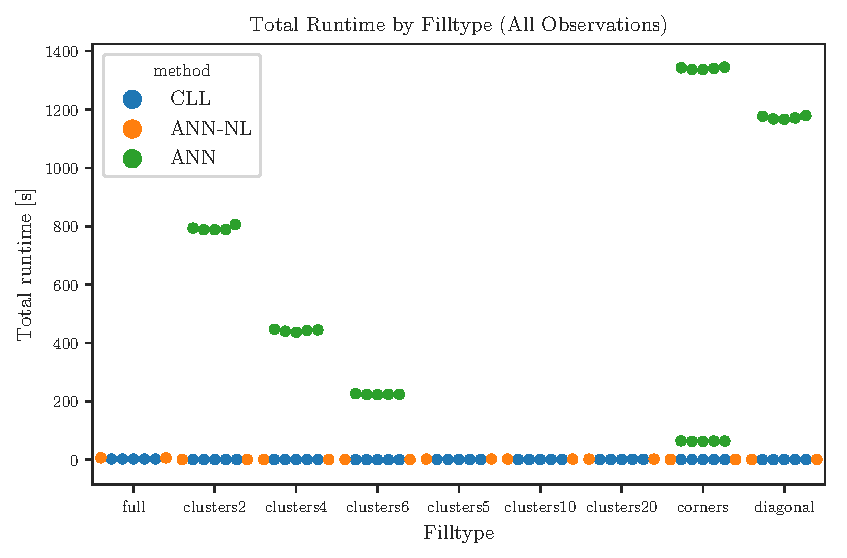
\includegraphics[width=\textwidth]{figures/totalruntime_all.pdf}
	\caption{FIXME!}
\end{figure}
\begin{figure}[h]
	\centering
	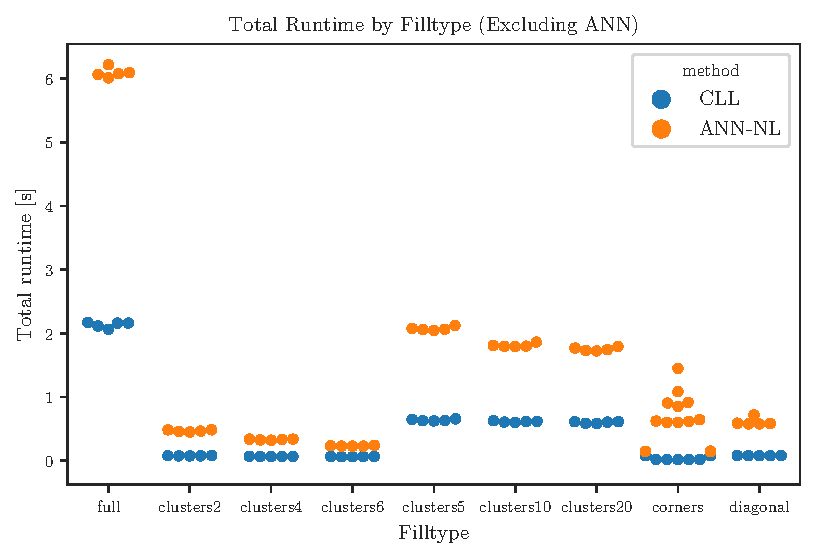
\includegraphics[width=\textwidth]{figures/totalruntime_noann.pdf}
	\caption{FIXME!}
\end{figure}



ann and list building in detail -> throw out

compare search times of ann and annnolist - compiler?

corners, compare across fills

11, compare across filltypes


Datenquelle nachvollziehbar und abgelegt

Einfüsse (Befüllungsgrad, Suche) einzelnd hervorheben


In diesem Kapitel werden die Ergebnisse beschrieben, diskutiert und ggf. mit anderen Daten aus der Literatur verglichen. Die Diskussion soll klären, ob die Daten sinnvoll sind, die Ergebnisse so zu erwarten waren und ob ungewöhnliche Beobachtungen sichtbar sind. Es ist auf eine übersichtliche Struktur zu achten, untersuchte Fälle sind konsistent und logisch zu benennen. Die Darstellung der Daten ist an die verwendete Messgenauigkeit anzupassen (z.B. ist eine Angabe von \SI{314.394575}{K} in den meisten Fällen nicht sinnvoll).
 
\chapter{Summary and Outlook}

Die Zusammenfassung ermöglicht Außenstehenden einen Überblick über den Inhalt der Arbeit und enthält insbesondere die Zielsetzung, die verwendete Methodik, Verfahren und Ansätze sowie die erzielten Ergebnisse. Daran schließt sich ein Ausblick an, der mögliche Verbesserungen bzw. weitere Arbeitsschritte aufzählt. Die Zusammenfassung ist das am häufigsten gelesene Kapitel (größt mögliche Sorgfalt!) und umfasst maximal zwei bis drei Seiten.


